\section{1174043 - Irvan Rizkiansyah}
	\subsection {Definisi Kecerdasan Buatan}
	Kecerdasan buatan atau biasa disebut AI (Artificial Intelligence) merupakan kecerdasan yang dibuat dan ditambahkan oleh manusia ke suatu sistem teknologi, yang diatur dan dikembangkan dalam konteks ilmiah, yang merupakan bentukan dari kecerdasan entitas ilmiah yang ada. Jadi pada intinya definisi AI dapat terus dikembangkan, namun yang menjadi poin utamanya adalah bagaimana manusia menciptakan sebuah teknologi yang dapat berpikir seperti selayaknya manusia itu sendiri.
	
	\subsection{Sejarah dan Perkembangan}
	\begin{itemize}
		\item Program kecerdasan buatan atau Artificial Intelligence pertama kali dicetuskan pada kisaran tahun 1951. Tidak bisa dipungkiri bahwa di tahun tersebut memang sedang gencar-gencarnya pembuatan cikal bakal, konsep, hingga teknologi berbasis AI. Dan, AI sendiri pertama kali digunakan di University of Manchester untuk menjalankan sebuah mesin bernama Ferranti Mark 1.
		\item Beberapa waktu kemudian, Christopher Strachey melanjutkan konsep kecerdasan buatan untuk menjalankan sebuah permainan catur, dimana bidak catur tersebut dapat berjalan secara otomatis dan mampu bermain melawan manusia sungguhan.
		\item Berlanjut pada tahun 1956, kecerdasan buatan tidak hanya dibuat untuk memudahkan bermain catur saja. Melainkan pada saat konferensi pertamanya, John McCharty menamai algoritma teknologi tersebut dengan sebutan “Artificial Intelligence”. Istilah tersebut masih digunakan hingga sekarang oleh para pakar teknologi.
		\item Terakhir, konsep dan teknologi kecerdasan buatan disempurnakan oleh seorang ahli yang namanya masih diingat sampai sekarang sebagai seorang pakar kecerdasan buatan, yaitu Alan Turin. Pada saat itu, Alan Turin meneliti dan menguji coba algoritma AI yang diberi nama dengan “Turing Test”. Hingga seiring berkembangnya waktu, konsep teknologi AI banyak digunakan di berbagai teknologi baik itu multimedia, search engine, dan masih banyak lainnya.
	\end{itemize}
	
	\subsection{Supervised Learning}
	Supervised learning (Pembelajaran terawasi), dalam konteks kecerdasan buatan (AI) dan Machine Learning, adalah jenis sistem di mana input dan output data yang diinginkan disediakan. Input dan output data diberi label untuk klasifikasi untuk memberikan dasar pembelajaran untuk pemrosesan data di masa depan.
	
	\subsection{Unsupervised Learning}
	Unsupervised learning merupakan pembelajan yang tidak terawasi dimana tidak memerlukan target output. Pada metode ini tidak dapat ditentukan hasil seperti apa yang diharapkan selama proses pembelajaran, nilai bobot yang disusun dalam proses range tertentu tergantung pada nilai output yang diberikan. Tujuan metode uinsupervised learning ini agar kita dapat mengelompokkan unit-unit yang hampir sama dalam satu area tertentu.
	
	\subsection{Teknik Klasifikasi}
	Teknik klasifikasi memprediksi respons diskrit, misalnya seperti apakah email itu asli atau spam, atau apakah tumor itu kanker atau tidak. Model klasifikasi mengklasifikasikan data masukan ke dalam kategori tersebut.
	
	\subsection{Regresi}
	Regresi yaitu pengeluaran nilai output yang konstan jika dipicu dengan parameter tertentu biasanya regresi disini berbentuk regresi linier. Regresi linier yaitu metode statistika yang digunakan untuk membentuk model hubungan antara variabel terikat(dependen,respon,Y) dengan satu atau lebih variabel bebas(independent, prdiktor, X). Apabila banyaknya variabel bebas hanya ada satu, disebut sebagai regresi linier sederhana, sedangkan apabila terdapat lebih dari satu variabel bebas, disebut sebagai regresi linier berganda.
	
	\subsection{Training Set}
	Training set adalah bagian dari dataset itu sendiri yang dilatih untuk membuat prediksi atau algoritma mesin learning lainnya sesuai keinginan atau tujuan data itu dibuat.
	
	\subsection{Testing Set}
	Testing set adalah bagian dari dataset yang di tes atau diujicoba untuk melihat keakuratannya dengan katalain melihat peformanya.
	
	\subsection{Instalasi dan Percobaan Kompilasi dari Library Scikit-learn}
	\begin{enumerate}
		\item Buka anaconda prompt
		\item kemudian Ketik di anaconda prompt yaitu : "pip install -U scikit-learn" \break
		\begin{figure}[H]
			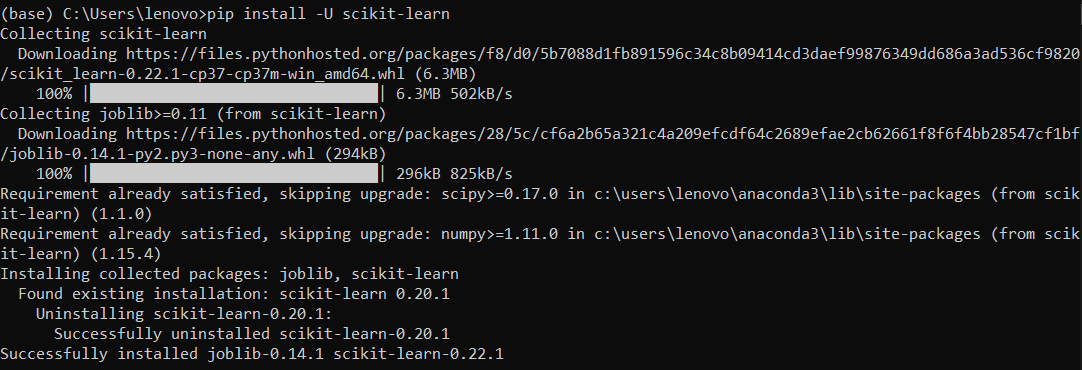
\includegraphics[width=4cm]{figures/1174043/chapter1/1.png}
			\centering
			\caption{Instalasi Scikit Learn}
		\end{figure}
		\item Setelah selesai instalasi, pilih salah satu example dari website Scikit
		\item Sample kode \break \lstinputlisting[firstline=1]{src/1174043/chapter1/sample1.py}
		\item Kemudian jalankan aplikasi tersebut, dan bisa dicek hasil dari Variable explorernya \break
		\begin{figure}[H]
			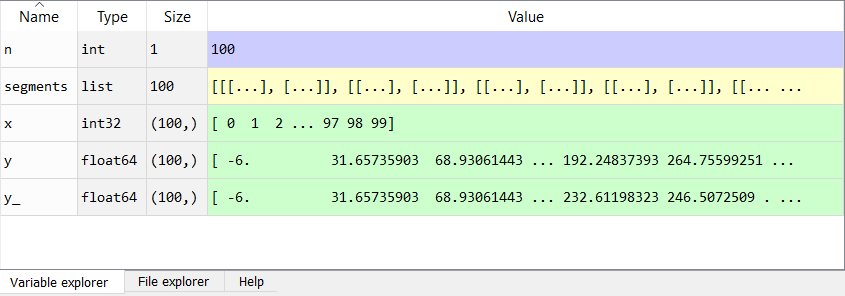
\includegraphics[width=4cm]{figures/1174043/chapter1/hasil_sample.png}
			\centering
			\caption{Variable Explorer}
		\end{figure}
	\end{enumerate}
	
	\subsection{Mencoba Loading an example dataset}
	\begin{enumerate}
		\item Sample kode \break \lstinputlisting[firstline=1]{src/1174043/chapter1/sample2.py}
		\item Kemudian jalankan aplikasi tersebut \break
		\begin{figure}[H]
			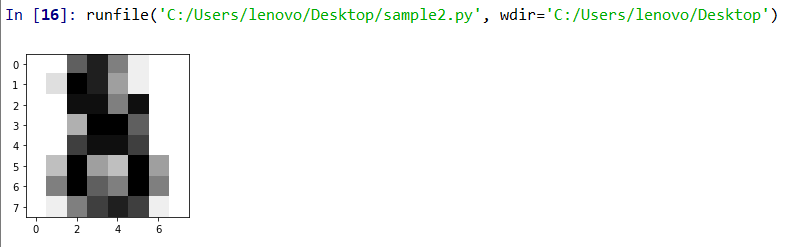
\includegraphics[width=4cm]{figures/1174043/chapter1/hasil_dataset.png}
			\centering
			\caption{Dataset}
		\end{figure}
	\end{enumerate}
	
	\subsection{Mencoba Learning and Predicting}
	\begin{enumerate}
		\item Sample kode \break \lstinputlisting[firstline=1]{src/1174043/chapter1/sample3.py}
		\item Kemudian jalankan aplikasi tersebut \break
		\begin{figure}[H]
			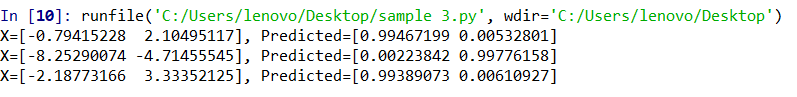
\includegraphics[width=4cm]{figures/1174043/chapter1/hasil_sample3.png}
			\centering
			\caption{Predicting}
		\end{figure}
	\end{enumerate}
	\subsection{Mencoba Model Persistence}
	Sample kode \break \lstinputlisting[firstline=1]{src/1174043/chapter1/sample4.py}
	
	\subsection{Mencoba Conventions}
	Sample kode \break \lstinputlisting[firstline=1]{src/1174043/chapter1/sample5.py}